\section{Schema termodinamico}
\label{sec:schema termodinamico}

\subsection{Analisi dello schema semplificato del sistema motore}
\label{subsec:schema semplificato}

Lo schema termodinamico semplificato del sistema propulsivo F-1 viene presentato di seguito. Per poter trattare le principali grandezze termodinamiche quali la pressione P, la temperatura T e la portata massica $ \dot{m} $, sono stati consultati i manuali del motore per poter estrapolare uno schema semplificativo a blocchi \cite{engine_manual}.
Nello schema presentato viene introdotto il sistema a ciclo generatore di gas che permette l’alimentazione della turbopompa. Supponendo il funzionamento a regime (Main Stage), l’alimentazione è completamente auto sostenuta finché non viene soppressa dai computer di bordo (al termine del $ t_{burn} $) o viene esaurito il propellente.

Qualitativamente, dai due serbatoi di LOX e RP-1 viene spillata una portata, che viene trattata dalla turbopompa per portare in pressione i due liquidi. I due tank sono messi leggermente in pressione da un gas inerte: elio (e GOX nel tank LOX).
Risulta vantaggioso avere un gas in pressione poiché permette un'uscita facilitata dai due tank ed evita la cavitazione man mano che essi vengono svuotati. La turbopompa sarà trattata in dettaglio nei paragrafi successivi, data la sua complessità costruttiva.
Ai fini dello schema proposto è sufficiente sapere che essa ha il compito di portare ad una certa pressione i due liquidi. Per poter alimentare le pompe, viene calettata sullo stesso asse in comune una turbina, la quale viene mossa da gas caldi combusti in una piccola camera di combustione.
Questo sottosistema viene chiamato Gas Generator (GG), e viene alimentato da una portata spillata dopo le turbopompe della stessa coppia RP-1/LOX, con un eccesso di combustibile per evitare temperature elevate all'ingresso della turbina.
I gas caldi in uscita dal GG vengono inoltre sfruttati per scaldare e quindi pressurizzare l’elio; successivamente tali gas di scarico vengono convogliati in un tubo circonferenziale all’ugello, nella posizione in cui il rapporto tra aree del divergente è pari a 10:1, dove vengono scaricati sulla parete interna dell’estensione dell’ugello.
Questo viene fatto per creare un film di gas relativamente freddi che hanno il compito di alleviare il carico termico sopportato dalla porzione finale dell'ugello (vedi -----APPENDICE----- per rappresentazioni grafiche dettagliate).
Il raffreddamento della parte superiore dell’ugello viene effettuato facendo passare il combustibile in diversi tubi esterni posti nella sezione tra gola e divergente 10:1; il combustibile riscaldato viene poi introdotto in camera di combustione.

In \autoref{table:dati_schema_termodinamico} e \autoref{fig:schema_termodinamico} si vedono alcuni dati rappresentativi dell'intero sistema. Si è ipotizzato di trattare i gas come perfetti e di assumere come dati alcuni rendimenti e alcune grandezze caratteristiche.

\begin{minipage}{0.4\linewidth}
    \centering
    \captionsetup{type=figure}
    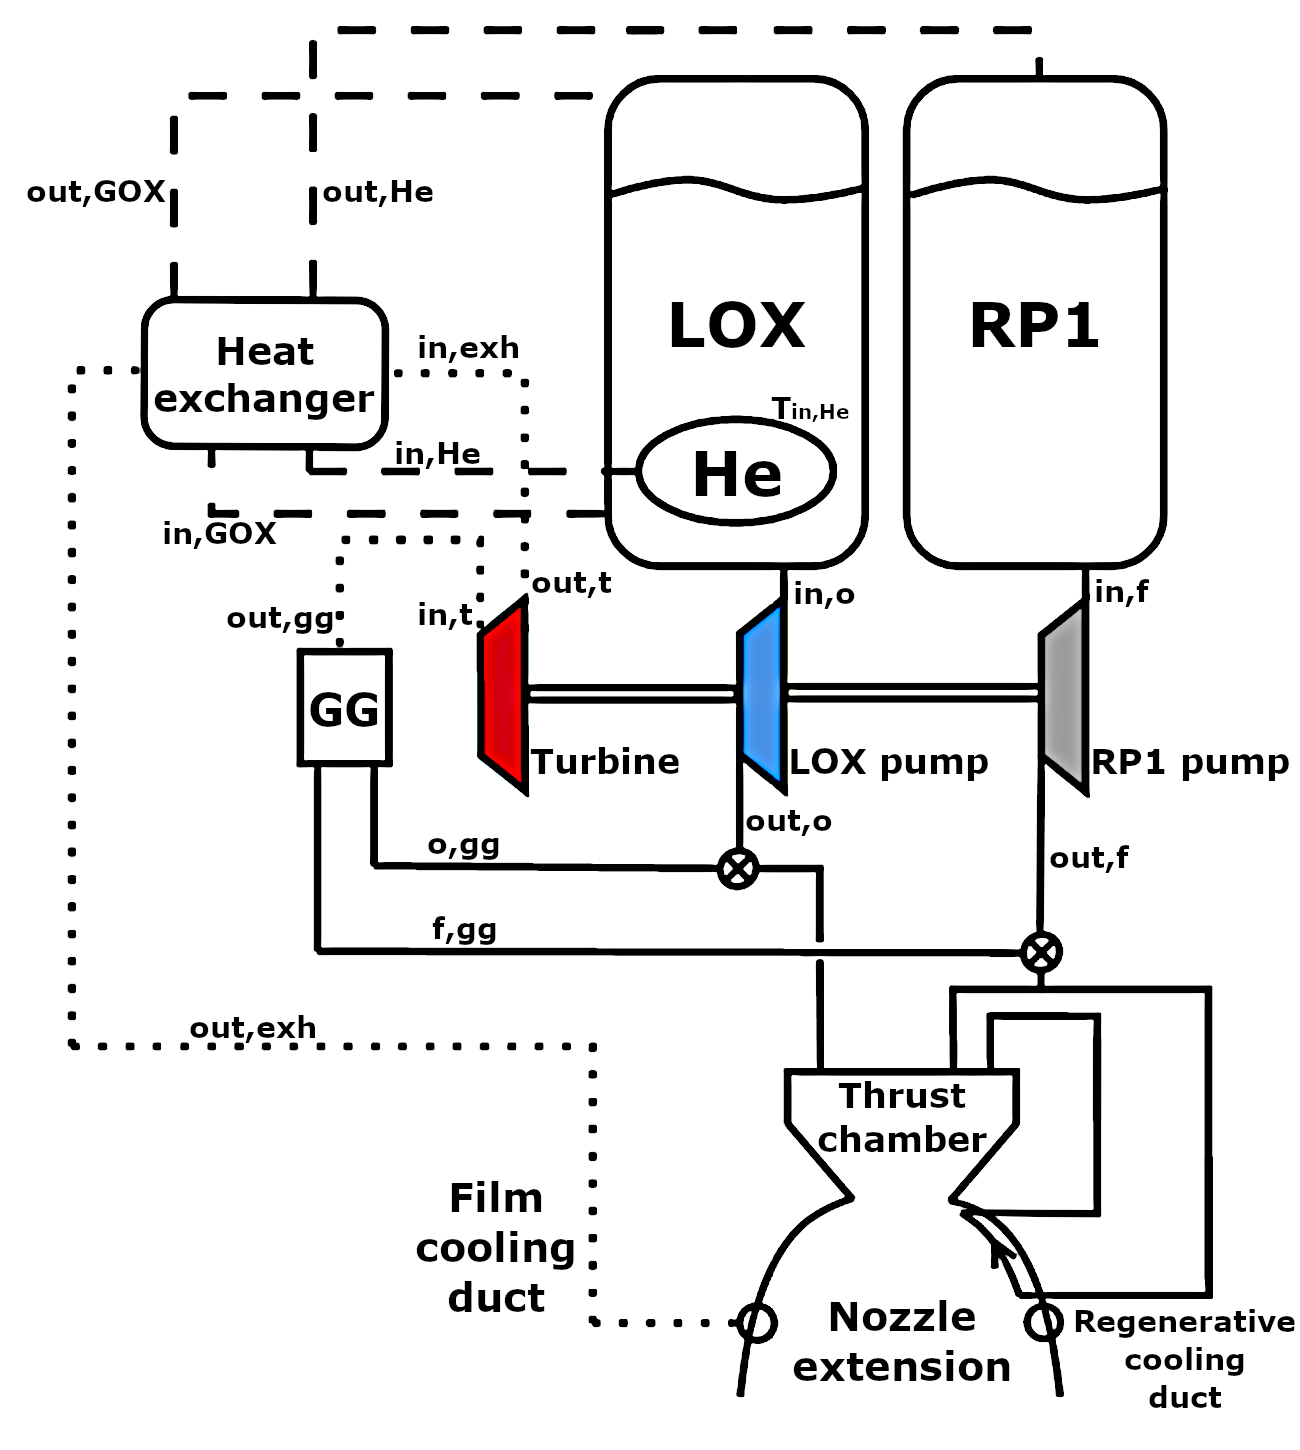
\includegraphics[width=\linewidth]{schema_termodinamico}
    \caption{Schema termodinamico}
    \label{fig:schema_termodinamico}
\end{minipage}\hfill
\begin{minipage}{0.6\linewidth}
    \centering
    \captionsetup{type=table}
    \scriptsize
    \renewcommand{\arraystretch}{2}
    \setlength\extrarowheight{-1pt}
    \begin{tabular}{|c|c|c|c|c|c|}
        \hline
        & $\bm{p_{in} \, [bar]}$ & $\bm{p_{out} \, [bar]}$ & $\bm{\dot{m}_{p} \, [kg/s]}$ & $\bm{T_{in} \, [K]}$ & $\bm{T_{out} \, [K]}$ \\
        \hline
        \textbf{RP1 pump} & $3.1026$ & $128.93$ & $849.13$ & $90.15$ & $90.15$ \\
        \hline
        \textbf{LOX pump} & $4.4816$ & $110.45$ & $1828.43$ & $298.15$ & $298.15$ \\
        \hline
        \textbf{GG} & $68.94$ & $66.63$ & $77.25$ & $1062$ & $1062$ \\
        \hline
        \textbf{Turbine} & $64.05$ & $3.93$ & $77.25$ & $1062$ & $888.38$ \\
        \hline
        \textbf{HH (He)} & $207.86$ & $-$ & $0.2268$ & $90.15$ & $433.15$ \\
        \hline
        \textbf{HH (OX)} & $96.52$ & $93.08$ & $3.1752$ & $95.37$ & $380.37$ \\
        \hline
        \textbf{HH (EXH)} & $-$ & $-$ & $77.25$ & $888.38$ & $879.17$ \\
        \hline
    \end{tabular}
    \caption{Dati schema termodinamico}
    \label{table:dati_schema_termodinamico}
\end{minipage}

\subsection{Analisi sulla scelta del ciclo di alimentazione}
\label{subsec:analisi ciclo alimentazione}

Per via della presenza di un sistema a turbopompe per l'alimentazione del propellente, è necessario scegliere il design ottimale per il ciclo di potenza che alimenterà la turbina e di conseguenza le due pompe stesse.
La scelta del tipo di ciclo di potenza ha ripercussioni sulla filosofia del design dell'intero impianto e la sua introduzione può implicare una variazione in termini di prestazioni del sistema motore.
Nel motore F-1 è stato scelto un ciclo di alimentazione a Gas Generator: risulta il sistema più leggero e semplice tra tutti, e data la ridotta complessità è il più economico in termini di sviluppi.
Inoltre, è l'unico ciclo di alimentazione tra i principali ad avere un flusso di gas in parallelo alla camera di spinta: questa peculiarità ha ripercussioni sulle prestazioni del motore.

Altri principali tipi di cicli di alimentazione sono l'\textit{Expander Cycle} e lo \textit{Staged Combustion Cycle}. Oltre a questi, diversi ne sono stati sviluppati con combinazioni di diversa complessità che però in alcuni casi hanno portato a migliorare notevolmente le prestazioni globali del sistema motore.
Nell'\textit{Expander Cycle} la turbina viene alimentata grazie al riscaldamento rigenerativo del combustibile attraverso le pareti dell'ugello (permettendo quindi anche il raffreddamento delle pareti).
Il fuel, che viene vaporizzato, espande in turbina e successivamente entra in camera di combustione. La temperatura in entrata alla turbina è limitata, non ci sono combustioni prima di essa: questo limita l'energia ricavabile dalla turbina e limita anche la pressione ottenibile in camera.
Il necessario cambio di fase è un fattore limitante nell'utilizzo di tale ciclo: al crescere della dimensione del motore bisogna aumentare la portata in turbina in modo da aumentare la potenza, ma tale portata è limitata da fattori geometrici, poichè deve passare nelle pareti dell'ugello ed essere adeguatamente portata a vaporizzazione.
Inoltre, la necessità di avere vaporizzazione immediata concentra l'utilizzo di questo ciclo per combustibili criogenici come l'idrogeno. Tale ciclo viene dunque usato per motori a spinte non troppo elevate e per stadi alti, e non poteva essere applicato al boost stage del primo stadio SI-C.

Nelle diverse tipologie di \textit{Staged Combustion Cycle} si introducono uno o più preburner in modo da suddividere la combustione in diverse zone, oltre alla camera di spinta principale.
Questo ciclo ha migliori prestazioni rispetto al ciclo a gas, poichè il flusso in uscita non viene scaricato in atmosfera ma introdotto nella camera principale. Questo aumenta l'efficienza del sistema, per contro lo sviluppo di questo ciclo aumenta notevolemente i costi e i tempi di sviluppo data la sua elevata complessità.
Per poter comprendere le difficoltà ingegneristiche da affrontare si deve riconoscere che in un ciclo chiuso non si potrebbe semplicemente scaricare i gas combusti del GG, dopo aver attraversato la turbina, direttamente in camera: la pressione troppo bassa in uscita dalla turbina non sarebbe compatibile con l'alta pressione richiesta dalla camera di spinta, e i prodotti di combustione di una miscela FR (Fuel Rich) di combustibili a idrocarburi come RP-1 provocherebbero difficoltà agli iniettori del piatto principale, intasandoli.
Da notare inoltre che nel ciclo chiuso FR tutto il fuel passa nel preburner, mentre nel gas generator vengono spillate delle piccole portate di fuel e oxidizer a monte. Questo implica che il sistema di preburner deve essere abbastanza grande da contenere una combustione controllata e generalmente a portate elevate di propellenti (a pressioni molto alte), soprattutto per quanto riguarda i booster stage.
Un altro accorgimento è la suddivisione in stadi della turbopompa del fluido che viene spillato (l'ossidante nel caso mostrato in \autoref{fig:staged_comb}). L'ossidante in questo caso deve essere pressurizzato ad alta pressione per la camera, e una sua piccola percentuale deve essere portata a quasi il doppio del valore di pressione di camera per entrare nel preburner.
Oltre a queste complicazioni, il ciclo chiuso FR non viene utilizzato con combustibili a lunga catena carboniosa come RP-1, per il problema legato ai suoi prodotti di combustione. Si preferisce usare questo ciclo con combustibili come idrogeno o metano (come nei nuovi motori sviluppati da SpaceX). I motori con cicli chiusi e OR (Oxidizer Rich), storicamente sviluppati dai russi dall'inizio degli anni '50, venivano alimentati anche con carburanti come il kerosene.

Concludendo, si può dire che la scelta del ciclo di alimentazione per il motore F-1 è ricaduta su un ciclo a gas per una combinazione di fattori, quali: esigenze prestazionali del singolo motore, elevate in termini di potenza e per quel tipo di combinazione di propellenti (con un trade-off sulla perdita di prestazione, come visto in seguito); limitazioni date dallo sviluppo degli altri cicli di alimentazione in quel periodo storico; minore complessità del sistema stesso.

\twofig{staged_comb}{Staged Combustion Cycle FR}{staged_comb}{full_cycle}{Staged Combustion Cycle completo}{full_cycle}

\subsection{Analisi delle variazioni di performance introdotte dal ciclo a gas}
\label{subsec:analisi performance ciclo a gas}

In questa sezione verrà analizzato come l'introduzione del ciclo a gas ha delle ripercussioni sulle performance del sistema stesso, in particolare sull'impulso specifico del sistema motore, che verrà denotato come $I_{s,oa}$ (l'abbreviativo \textit{oa} si riferisce al termine "overall"). Importante è la distinzione tra l'impulso specifico del motore intero (appena introdotto) e quello della camera di spinta (più ugello), che sarebbe quello teorico e denotato come $I_{s,tc}$.

Per poter trattare teoricamente le limitazioni, si parte dal presupposto che a parità di altri fattori (come quota, mixture ratio, rapporto di espansione, ecc.) un aumento di pressione in camera di combustione aumenta le prestazioni del sistema. Infatti, analizzando la spinta si vede che:
\begin{empheq}{equation*}
T = \dot{m}_p u_e + A_e \left( p_a - p_e \right)
\qquad \text{dove} \qquad
u_e = u_e \left( p_c \right) = \sqrt{\frac{2 \gamma R T}{\gamma - 1} \left[ 1 - \left( \frac{p_e}{p_c} \right) ^ {\frac{\gamma - 1}{\gamma}} \right]}
\end{empheq}

Si nota come aumentando la pressione in camera, a questo livello di approssimazione, la spinta aumenta indefinitamente, per cui anche l'impulso specifico $I_{s,tc}$ aumenterà poichè esso è definito da:
\begin{empheq}{equation*}
I_{s,tc} = \frac{T \left( p_c \right)}{\dot{m}_p} = u_e \left( p_c \right) + \frac{A_e \left( p_a - p_e \right)}{\dot{m}_p}
\end{empheq}

Questo ci permetterebbe di concludere che un aumento di pressione illimitato in camera di combustione aumenta indefinitamente le prestazioni, sia perchè l'ugello può espandere a pressione più alta, sia per il contributo statico.
Introducendo però un sistema di alimentazione di potenza in parallelo come il GG, si ha in realtà un calo di prestazioni rispetto all'andamento teorico.

Questo fatto può essere compreso a livello qualitativo considerando che, in un tale sistema, aumentare la pressione in camera significa aumentare le prestazioni richieste dalle pompe, richiedendo quindi più potenza dalla turbina.
A parità di salto di pressione in turbina e prodotti di combustione del GG, l'unico modo che si ha per aumentare la potenza prodotta dalla turbina è aumentare lo spillamento di portata dal flusso che andrà poi in camera.
Questo flusso, oltre a non conseguire una combustione ottimale (ovvero con rapporto O/F molto diverso da quello della camera), viene espanso a velocità molto più basse e questo implica una perdita di prestazioni che può essere quantificata nel modo seguente \cite{AIAA_book_1}:

\begin{empheq}{gather*}
I_{s,oa} = \left( 1 - \frac{\dot{m}_{gg}}{\dot{m}_p} \right) I_{s,tc} + \frac{\dot{m}_{gg}}{\dot{m}_p} I_{s,gg}
\\
I_{s,gg} = I_{s,gg} \left( u_{e,gg}, \, p_{c,gg}, \, \dot{m}_{gg} \right)
\\
u_{e,gg} = u_{e,gg} \left( p_{c,gg} \right) = \sqrt{\frac{2 \gamma_{gg} R_{gg} T_{gg}}{\gamma_{gg} - 1} \left[ 1 - \left( \frac{p_{e,gg}}{p_{c,gg}} \right) ^ {\frac{\gamma_{gg} - 1}{\gamma_{gg}}} \right]}
\\
p_{c,gg} = 0.85 \cdot p_{c,tc}
\\
\dot{m}_{gg} = \dot{m}_{gg} \left( \text{pwr}, \, \eta_t, \, \epsilon, \, T_{in}, \, c_{p,gg} \right) = \frac{\text{pwr}}{\eta_t \, c_{p,gg} \, T_{in} \, \epsilon}
\\
\text{pwr} = \text{pwr}_{LOX} + \text{pwr}_{RP1} = \frac{\Delta p_{LOX} \, \dot{m}_{LOX}}{\eta_{p,LOX} \, \rho_{LOX}} + \frac{\Delta p_{RP1} \, \dot{m}_{RP1}}{\eta_{p,RP1} \, \rho_{RP1}}
\\
I_{s,tc} = I_{s,tc} \left( u_{e,tc}, \, p_{c,tc}, \, \dot{m}_{tc} \right)
\\
u_{e,tc} = u_{e,tc} \left( p_{c,tc} \right) = \sqrt{\frac{2 \gamma_{tc} R_{tc} T_{tc}}{\gamma_{tc} - 1} \left[ 1 - \left( \frac{p_{e,tc}}{p_{c,tc}} \right) ^ {\frac{\gamma_{tc} - 1}{\gamma_{tc}}} \right]}
\\
\dot{m}_{tc} = \dot{m}_p - \dot{m}_{gg}
\end{empheq}

Si è ipotizzato, come best practice, che la pressione in camera del GG sia l'85\% della pressione nella camera principale. Si ipotizza inoltre, in prima approssimazione, che il salto di pressione attraverso le pompe sia proporzionale alla pressione in camera, con costante di proporzionalità ottenuta dalla divisione delle due quantità note: prevalenza della pompa (sia LOX che RP-1) e pressione in camera nominale dell'F-1 \cite{AIAA_book_1}.
Sono state implementate tali equazioni in MATLAB, imponendo un range esteso di pressioni, per poter notare l'effetto dell'introduzione del gas generator nel sistema.

\cfig{I_spec_see}{Confronto tra impulsi specifici a livello mare}{I_spec_see}{0.6}

Si nota come, al valore di pressione associato al motore F-1, ci sia un calo di prestazione rispetto al teorico. Il valore di impulso cala da 291 secondi a circa 285 secondi (a livello mare). Questo modello non considera perdite prestazionali dovute al flusso 3D (con eventuali separazioni asimmetriche e considerazioni sulle onde d'urto): in questa situazione l'ugello è in condizione sovra-espansa. Queste perdite sono successivamente considerate nella modellazione tramite il software RPA.

Dai grafici precedenti si nota anche come l'ottimo prestazionale per l'impulso specifico del sistema complessivo sia a pressioni in camera molto elevate (attorno ai 30 MPa, ovvero 300 bar). Un valore di pressione così elevato richiede una revisione di tutti i sistemi di alimentazione, a partire dalla turbopompa. Tale valore di pressione si trova tuttora nei motori LRE di nuova generazione come il Raptor, che tra l'altro non possiedono il ciclo a gas.